\section{HAL}
\label{exo:hal}
\begin{refsection}[exos/hal.bib]

keywords: model-based control; predefined gait trajectory; strength augmentation; rehabilitation.\\

The hybrid assistive limb (HAL) exoskeleton is developed by the University of Tsukuba and Cyberdyne for human strength augmentation and as an assistive gait device in rehabilitation.  Although several prototypes have been developed, this section focuses on the most recent HAL-5 model (specifically the non-clicial type, HAL-5 Type-B). Though HAL-5 is a full body exoskeleton, only hip, knee joints, and ankle are actuated in the sagittal plane.  The exoskeleton powers DC motors with harmonic drives at hip, knee, ankle joints (in some models the ankle joints act as passive springs).  HAL weighs 23kg, includes an on-board AC100V battery as the power source, which is designed to support the power requirements of maximum velocity human walking and standing torque requirements.  The battery allows for 160 min of continuous operation and enables the exoskeleton to lift up to 70kg \cite{HALassist2011}.  

Human operators attach to HAL at the waist by a belt, and at the calf and thigh using harness. HAL's frame does not transfer load to the ground.  Instead, HAL adjusts hip, knee and ankle torques to amplify its operator's torque. The exoskelton's sensory system includes bioelectric sensing (including sEMG), angular sensors, acceleration sensors, and center of pressure / center of gravity (COP/COG) sensors.  COP/COG sensing is provided through shoes with ground reaction force sensors.  The joint measurements are provided by potentiometers.
In at least one version of HAL the bioelectric data comes from sEMG sensors installed below the operator's hip and above the knee (on both front and back).
An IMU installed in HAL's backpack is used to estimate torso pose.


\begin{figure}[ht]
  \centering
  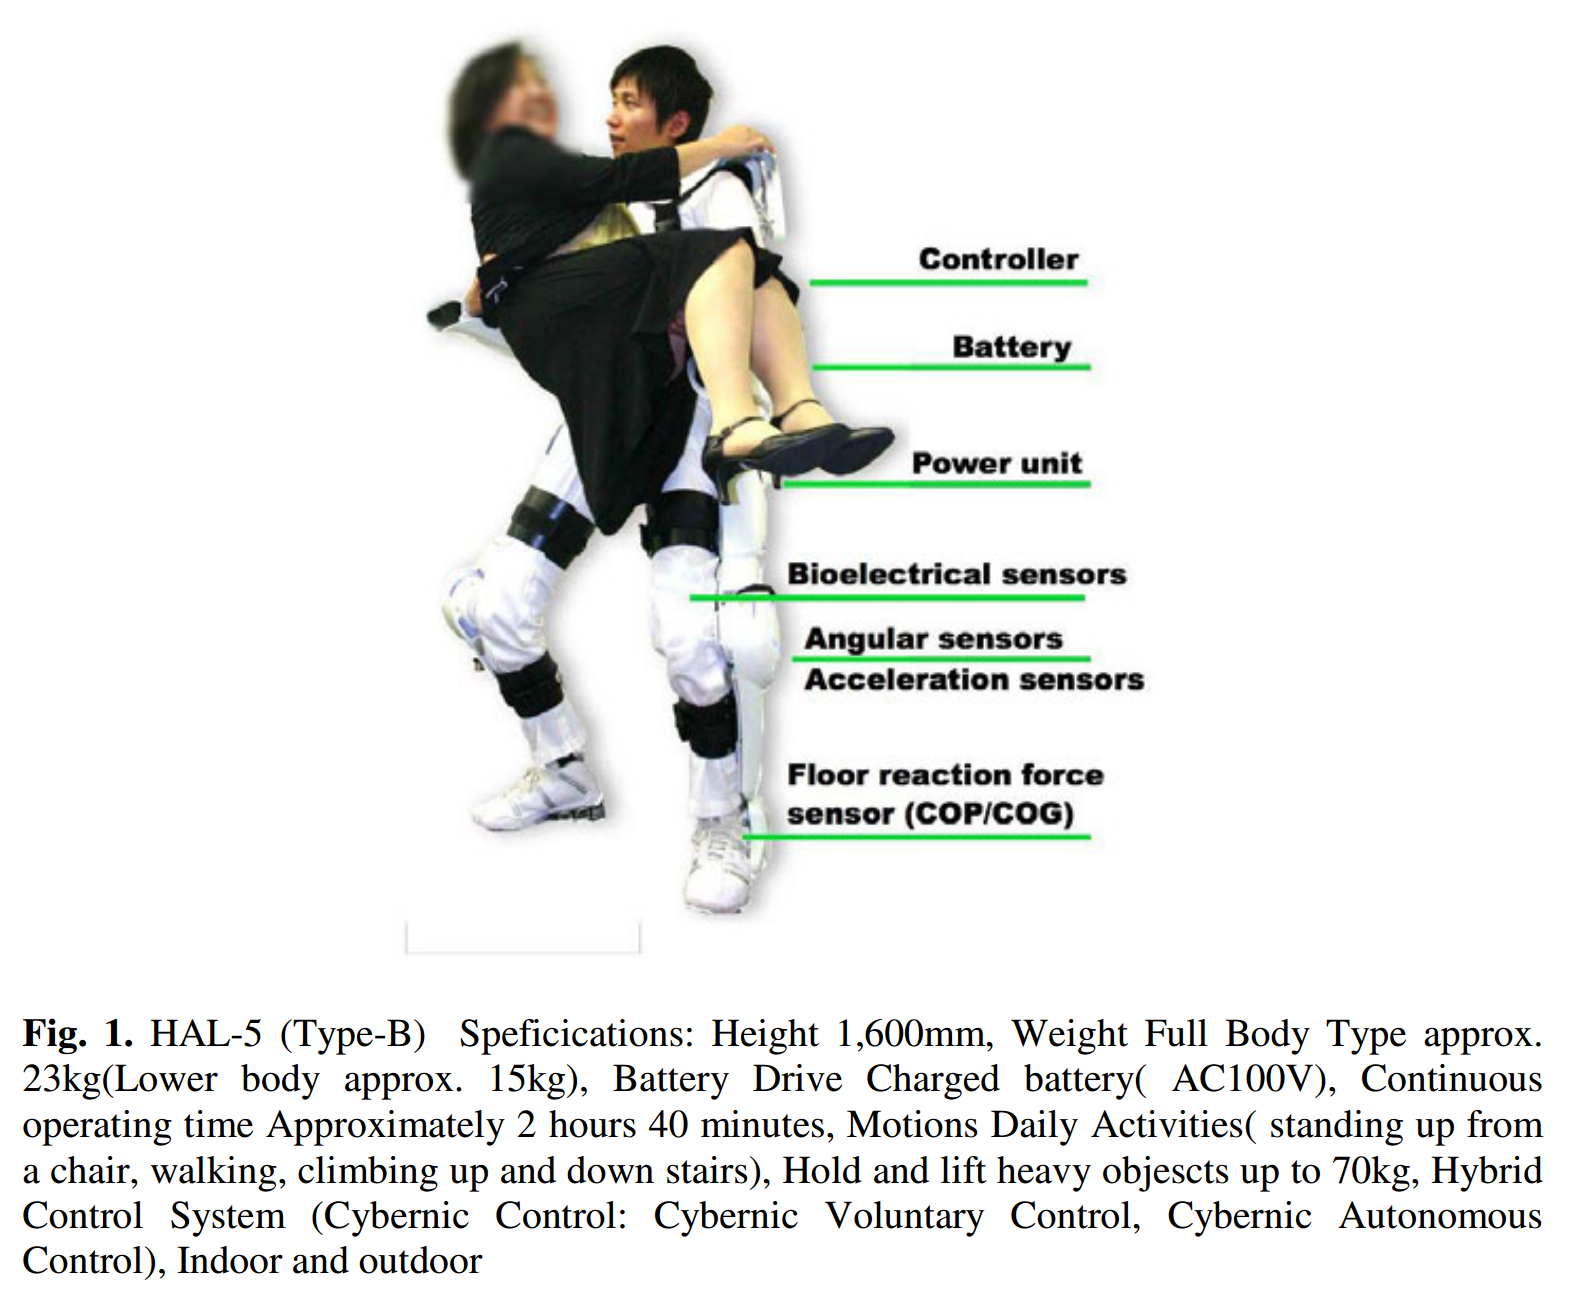
\includegraphics[width=3.5in]{exos/figs/hal-5_B_diagram.png}
\end{figure}


\subsubsection{Control}

HAL uses two types of control systems depending on application domain.  For gait assistance and rehabilitation, HAL uses an autonomous control system that carries the user through predefined gait trajectories by controlling knee and hip joints (the ankles behave as passive springs).  Gait phase intention is estimated from COP/COG sensors.  The exoskeleton drives the wearer to follow pre-recorded desired joint patterns.

The second control strategy, a model-based approach for human strength augmentation, estimates human intention from sEMG activity and provides power to augment torque provided by the operator.  A relatively autonomous torque assist strategy in \cite{HALmodelControlKnee2010} recognizes user intention to take a step by thresholding sEMG data.  The approach provides a knee torque response including an assitive torque component, a viscous damping component that reduces high velocity motion for safety, and a gravity compensation torque.  
%In \cite{HALvTorqueImp2002}, HAL uses myoelectric data to estimate muscle torque based on the difference between flexor and extensor muscle activities.  

In \cite{HALmuscleImped2005}, an impedance control strategy controls the viscoelastic properties of HAL's knee joint from a musculoskeletal model of operator's limb moving in concert with the exoskeleton.  The controller uses sEMG sensor data to estimate muscle torque based on the difference between flexor and extensor muscle activities.  The authors note the sEMG model requires significant calibration effort.  
%
\begin{figure}[ht]
  \centering
  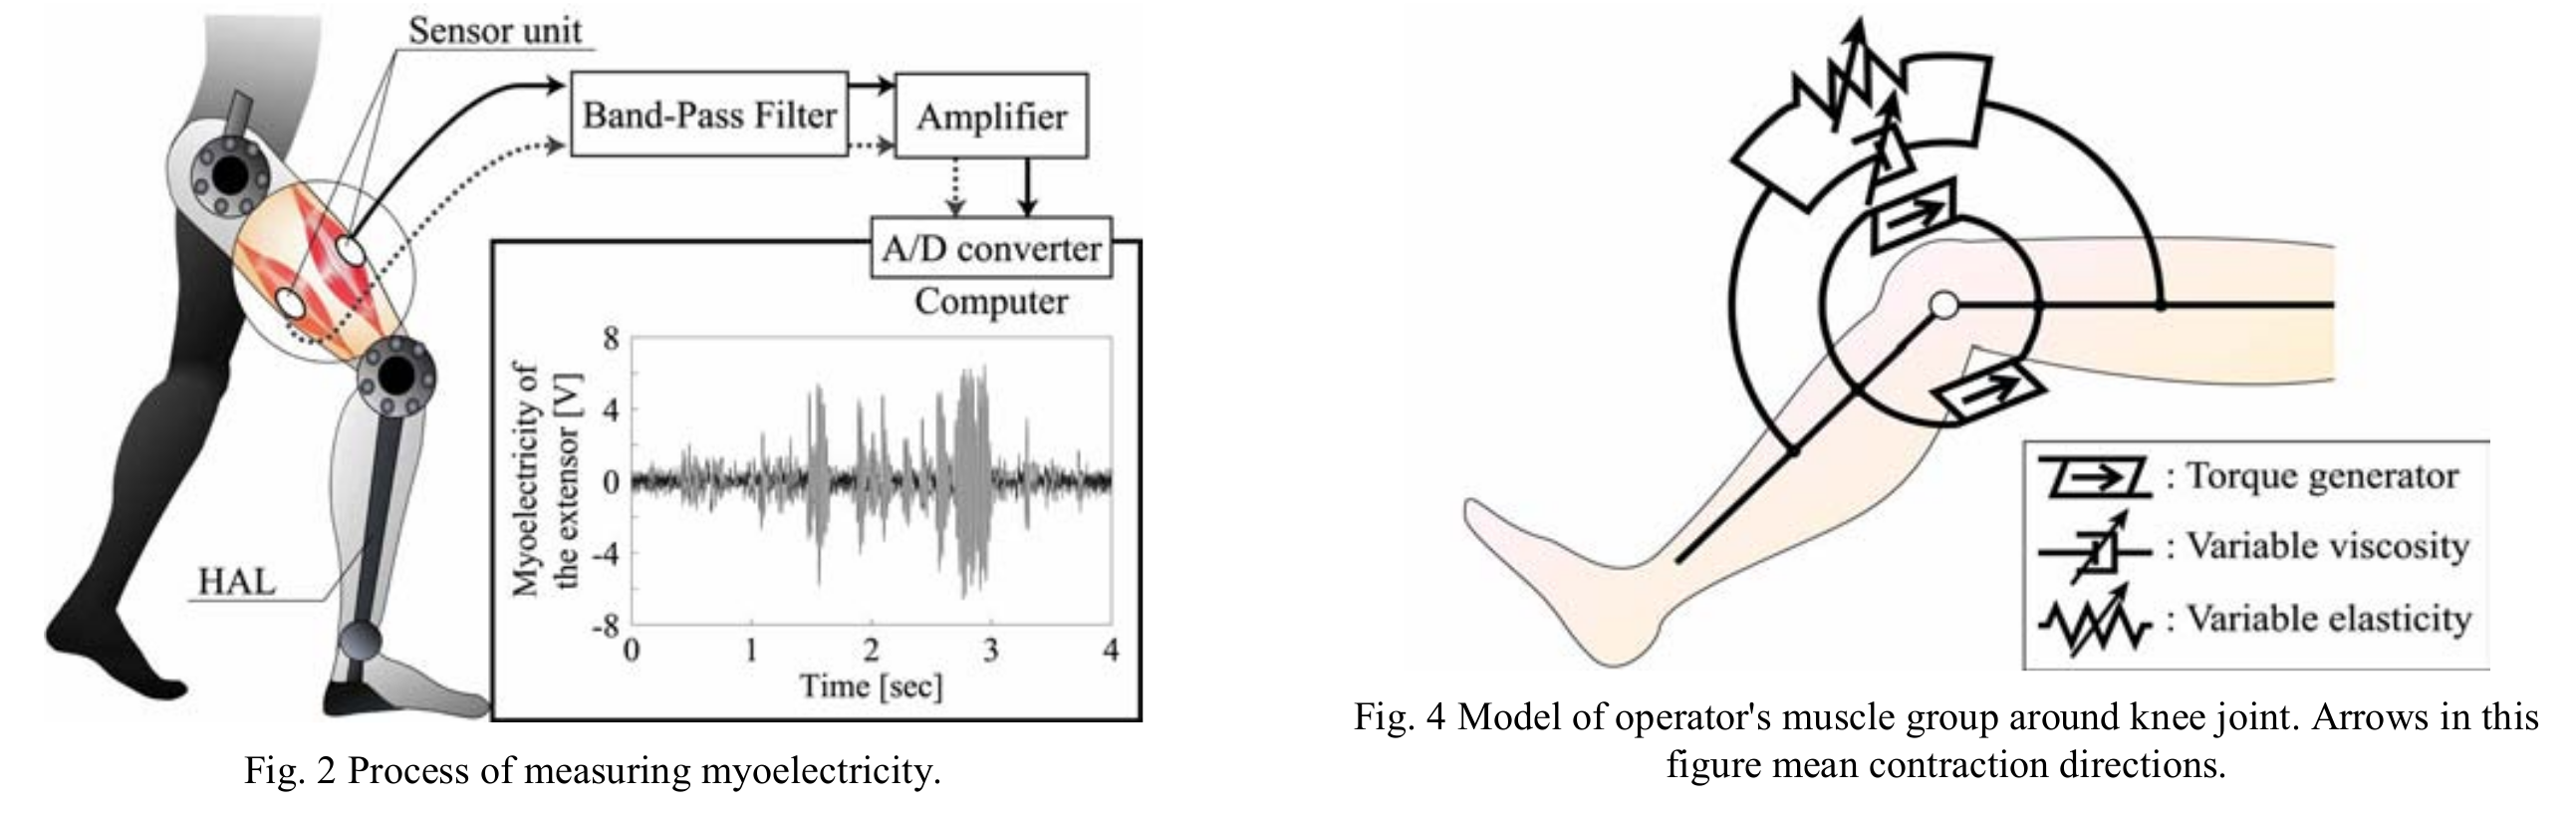
\includegraphics[width=6in]{exos/figs/hal_viscoelastic_control.png}
\end{figure}
%
%
Viscoelastic torques are computed according to
\[\tau_{a,i} = \alpha_i(-D_i \theta_i - K_i \theta_i),\]  
based on a variable gain set by $\alpha_i$.  The net knee actuator torque is
\[\tau_i = \tau_{a,i} + \tau_\mu + \tau_c .\]
The torque includes a $\tau_c$ term compensating for mechanical (actuator) impedance and $\tau_\mu$, a scaled version of the human torque (as estimated  from sEMG data).  The $K_i$ and $D_i$ terms in $\tau_{a,i}$ are viscoelastic parameters (based on the operator's muscles) in the human-exoskeleton model.  These parameters are estimated on-line using a weighted least-squares method.  In this case, the angular velocity data required for the impedance controller is estimated from a state observer.

While experiments in \cite{HALmuscleImped2005} only consider leg swing-up and swing-down, a similar control approach in \cite{HALvTorqueImp2002} switches the dynamics based controller to compensate for swing and stance phases in walking gait.  In this case, the gait transitions are detected by thresholding foot sensors and required angular velocity (and acceleration) data is determined by numerically differentiating angular encoders.


\subsection{Assessment and Recommendations}

Compared to sensitivity amplification methods, HAL's use of EMG data allows it to estimate intention without amplifying external disturbances.  This is ideal for combat scenarios.  However, sEMG data is extremely difficult to work with due to high filtering and calibration requirements.  A hybrid strategy which uses sensitivity amplification and sEMG data (possibly thresholded) to filter user intention could prove effective.  As an alternative, research into nano-fabrication and MEMs technologies has produced new ``robotic skin'' sensing arrays. This technology may allow direct measurement of interaction forces (i.e. estimating pressure / force and exoskeleton contact locations), which has not been feasible in the past.  Such measurements could (potentially) filter external disturbances from user generated input to estimate intent.

\nocite{*}
\printbibliography[heading=subbibliography]

The figures in this section were obtained from \cite{HALmuscleImped2005,HALassist2011}.  Materials presented are based on the references above.

\end{refsection}